\newpage
\section{Einleitung}
\begin{wrapfigure}[16]{r}{8.5cm}
	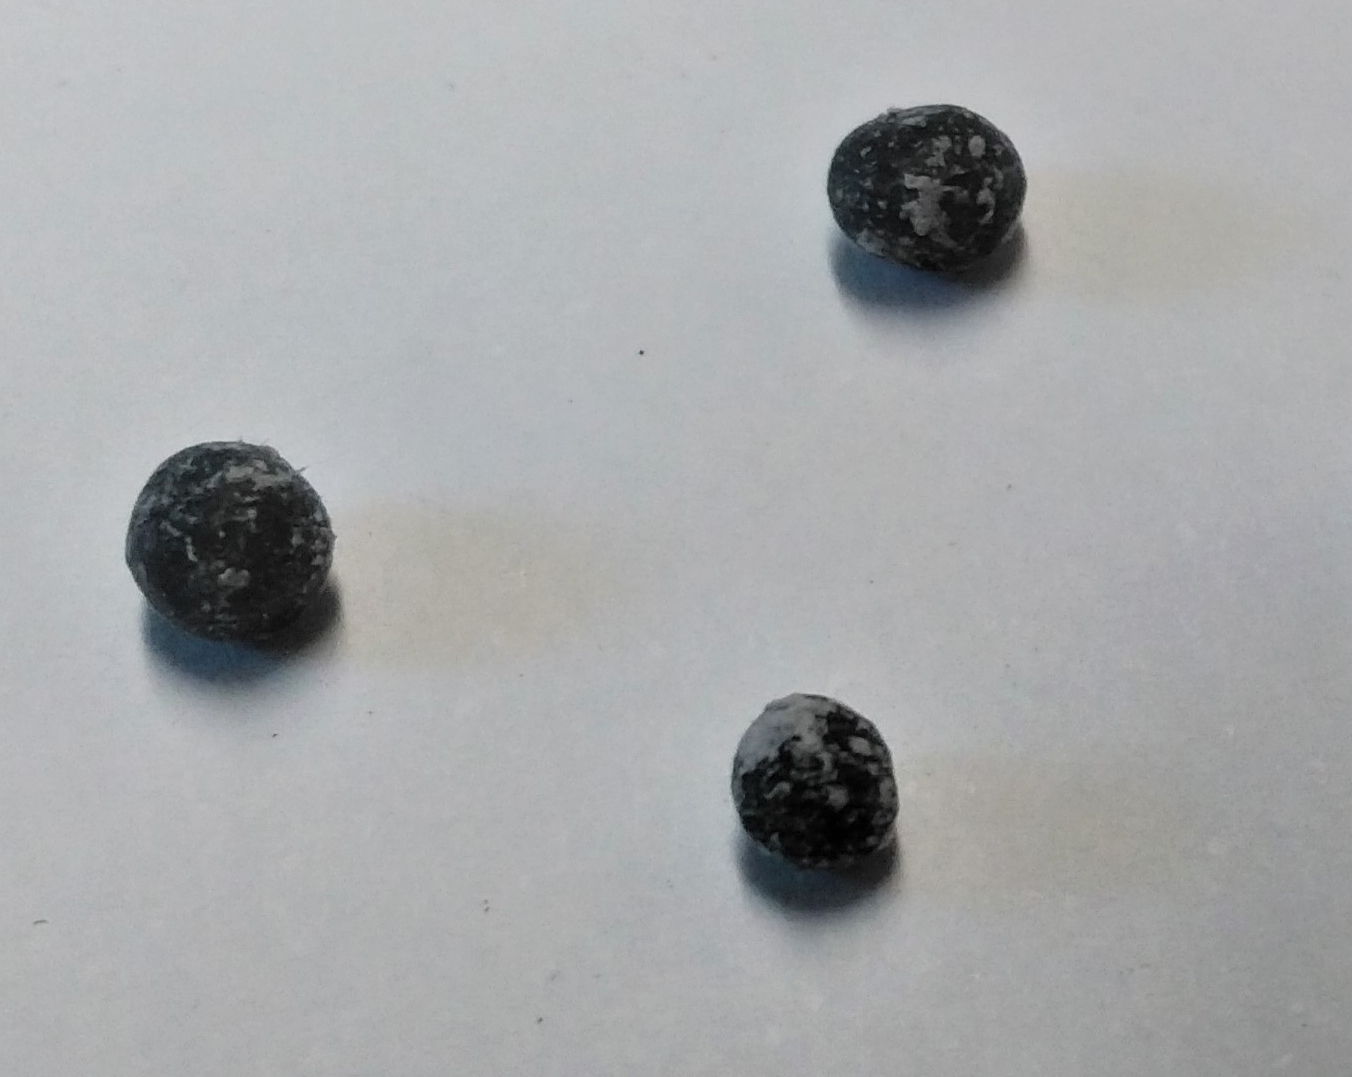
\includegraphics[scale=0.18]{Illustrationen/3-Einleitung/nemacaps.jpg}
	\caption{NemaCaps}
	\label{fig:nemacaps}
\end{wrapfigure}
\textit{(ygu)}Das Unternehmen MCC Laboratoire Meiners GmbH beschäftigt sich mit der Herstellung von Mikroverkapslungen. Neben der Pharma- und Kosmetikbranche werden Mikroverkapselungen auch in der Landwirtschaft eingesetzt. Für diese Branche entwickelt MCC Laboratoire Meiners GmbH Kapseln, sogenannte NemaCaps, welche in der biologischen Schädlingsbekämpfung eingesetzt werden. Ein NemaCap beinhaltet mehrere tausend Fadenwürmer (Nematoden). Neben Nematoden ist der Kapsel ein Schlafmittel beigemischt, sodass die Fadenwürmer schlafend gestellt sind. 
\newline
NemaCaps werden im Erdreich, im Wurzelbereich der zu schützenden Pflanze platziert. Durch den Regen oder das Begiessen der Pflanzen wird das Schlafmittel verdünnt und die Nematoden aktiv. Die Hülle der Kapseln besteht aus \textbf{XYZ}, welches elastische Eigenschaften besitzt und die Voraussetzung für das Durchbrechen der Fadenwürmer bildet. 
\newline
In ihrer natürlichen Umgebung angelangt, stossen die Fadenwürmer nun zufällig auf Larven von Schädlingen. Gemäss dem Nationalen Forschungsprogramm 68 [nachfolgend NFP 68]\cite{nfp} dringen die Nematoden durch die Körperöffnungen der Larven ein (Siehe Abb.  \ref{fig:zyklus_Nematoden}, Punkt 3). Im Körper der Larve angelangt, setzen die Fadenwürmer Bakterien ab (Punkt 1 in Abb.  \ref{fig:zyklus_Nematoden}). Diese Infektion führt innerhalb von 1-2 Tagen zum Tod des Insekts \cite{e-nema}. Die Fadenwürmer vermehren sich in der Larve bis diese komplett aufgezehrt ist \cite{nematoden}. Anschliessend verlassen die Nematoden den Kadaver und befallen weitere Larven. So beginnt der Kreislauf von Neuem (Punkt 2 in Abb.  \ref{fig:zyklus_Nematoden}).
\newline

\begin{wrapfigure}[10]{r}{7cm}
	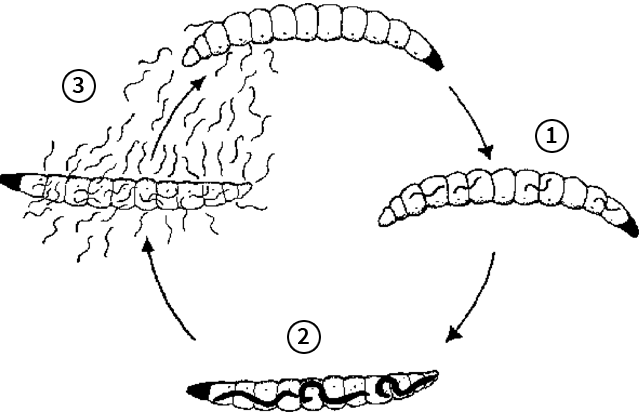
\includegraphics[scale=0.4]{Illustrationen/3-Einleitung/zyklus_nematoden.png}
\caption{Bekämpfung einer Larve durch Nematoden \protect\cite{e-nema}}
\label{fig:zyklus_Nematoden}
\end{wrapfigure}

	
Nematoden dienen speziell in der Bekämpfung von Wurzelschädlingen als wirksame Alternative zu Pestiziden. Pestizide können im Wurzelbereich weniger gezielt eingesetzt werden \cite{nfp}. Diese Überlegenheit möchte man durch den Einsatz von NemaCaps im Wurzelbereich nutzen. Durch die Kapselung ist eine gezielte Platzierung, Dosierung und verbesserte Handhabung von Nematoden möglich. Weiter werden durch die NemaCaps die Lagerung, Haltbarkeit un der Transport der Fadenwürmer vereinfacht. Diese Vorteile unterstreichen das Potential von NemaCaps, der biologischen Alternative von Pestiziden.
